\subsection{Der Messprozess}
	System $S$, Messaparat $M, M'$, Beobachter $B$
	
	Heisenbergscher Schnitt
		\begin{align*}
			S &| M, M', B,& S,M &| M', B,& S, M, M' &| B 
		\end{align*}
	Schnitt ist verschiebbar
		\begin{align*}
			\hat{A} \ket{a_n, j} &= a_n \ket{a_n, j}
		\end{align*}
	Oft nehme ich keine Entartung an: 
		\begin{align*}
		\hat{A} \ket{a_n} &= a_n \ket{a_n}
		\end{align*}
		\begin{align*}
			\ket{\psi} &= \sum_m c_m \ket{a_m}, & c_m &= \braket{a_m | \psi}
		\end{align*}
	\begin{figure}
		\begin{center}
			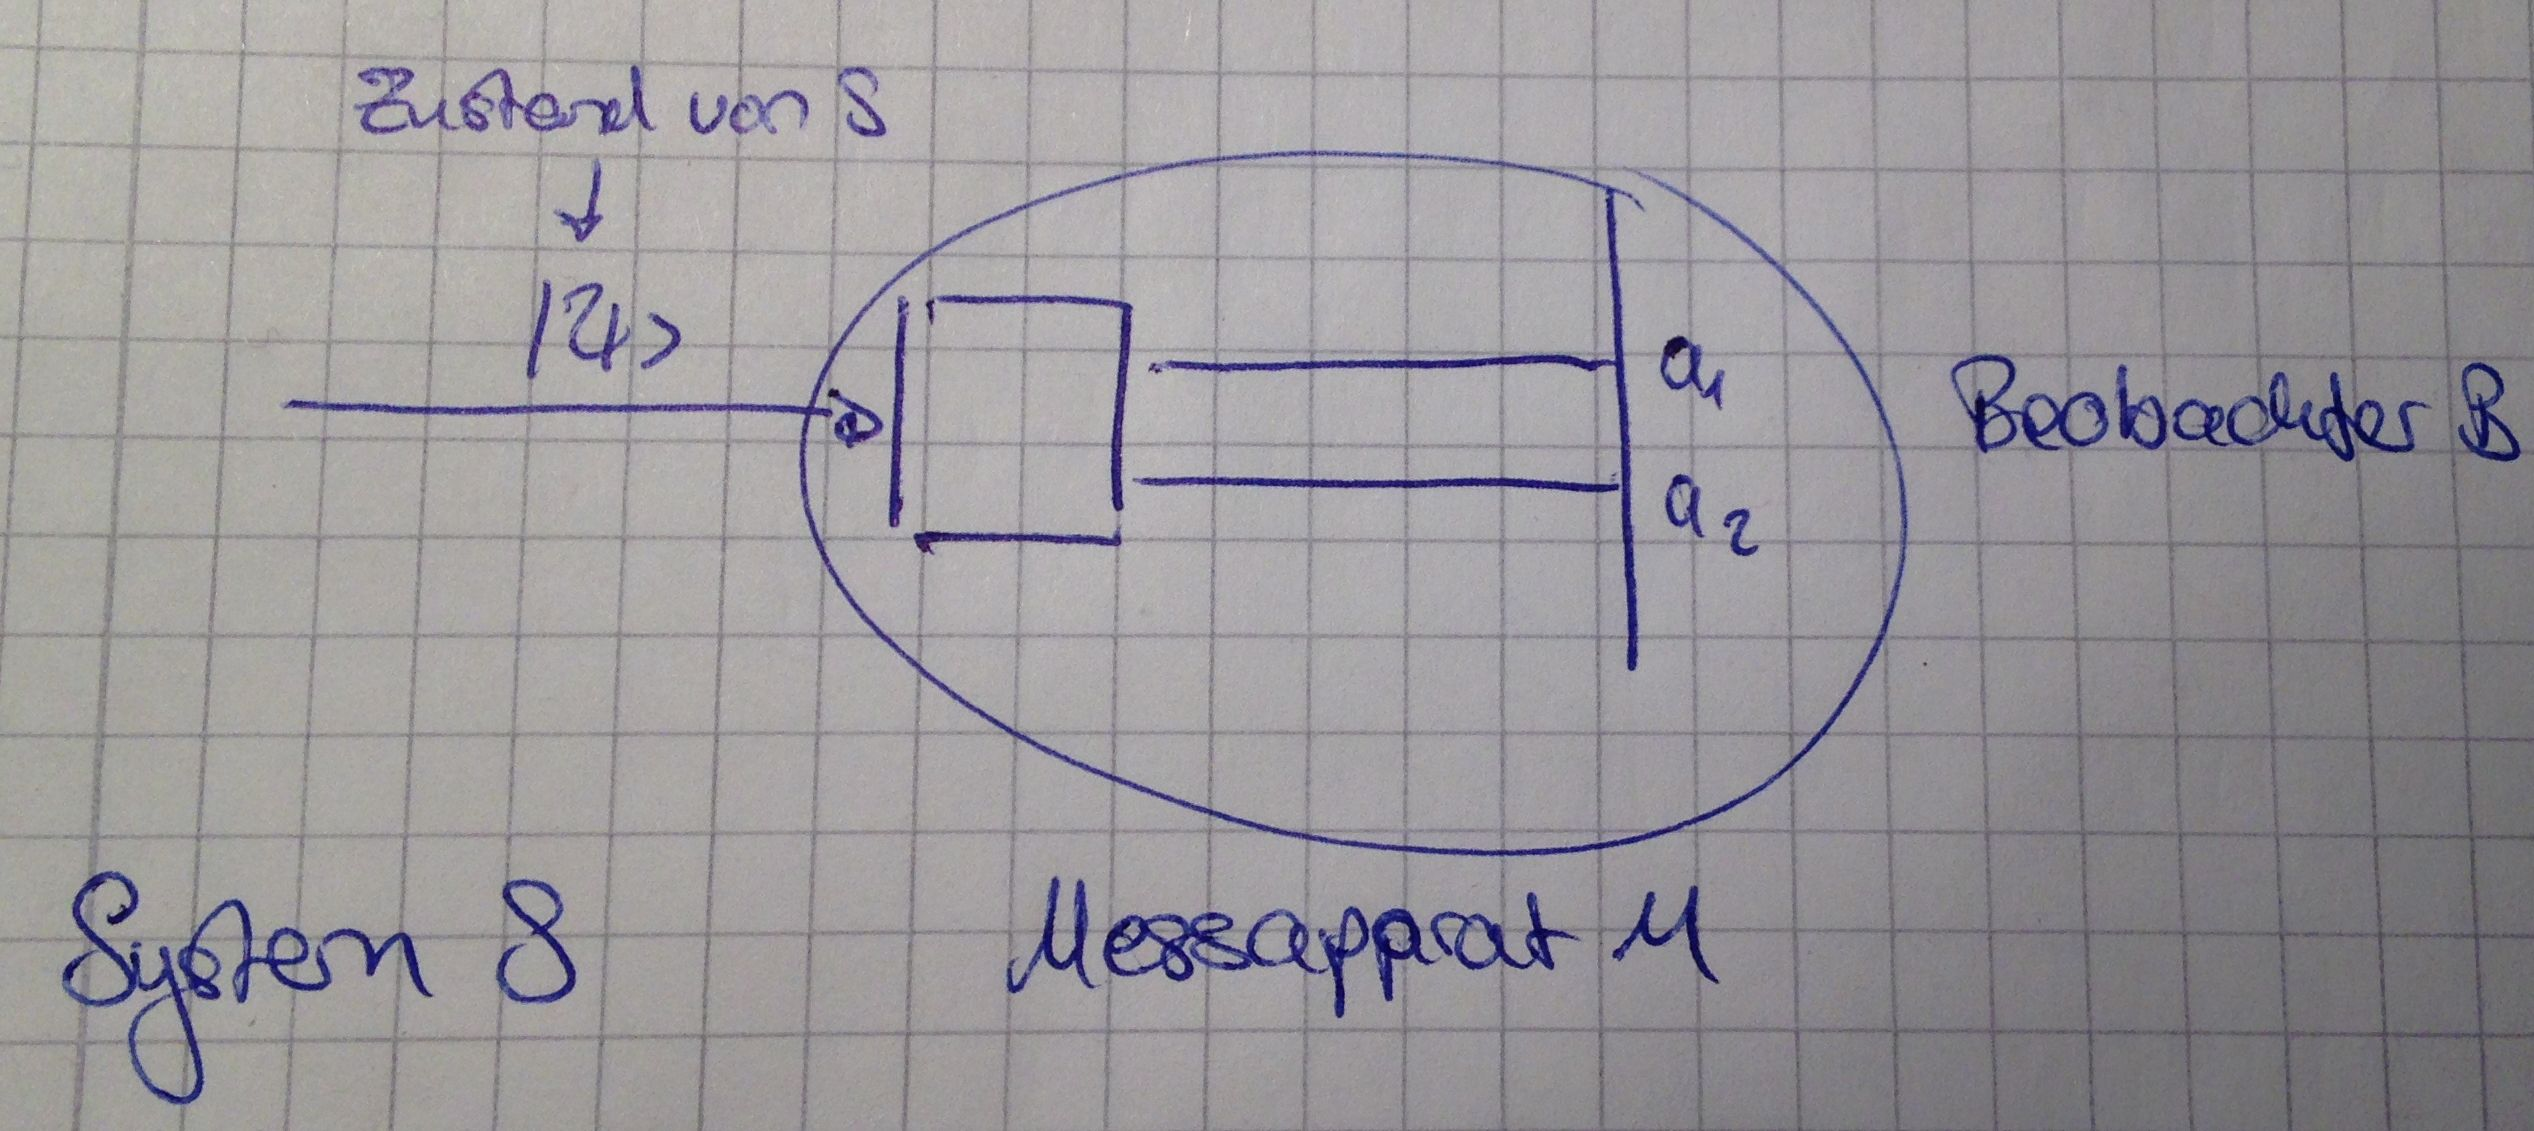
\includegraphics[width=0.7\textwidth]{Messung1}
		\end{center}
	\end{figure}
	
	Vor der Messung: 
		\begin{align*}
			\hat{\rho}_0 &= \ket{\psi} \bra{\psi} = \hat{P}_{\ket{\psi}}
		\end{align*}
	Nach der Messung ist System in einem Zustand
		\begin{align*}
			\ket{a_m} (\text{oder } \sum_{j = 1}^{d(m)} d_j \ket{a_m, j})
		\end{align*}
	auch bevor $B$ das Ergebnis abgelesen hat.
	
	Wahrscheinlichkeit des Messwertes (z.B. der Zeigerstellung)
		\begin{align*}
			a_m \text{ ist } W_m &= |c_m|^2 = \mathrm{Sp}\, (\ket{\psi} \bra{\psi} P_m) = 
			\mathrm{Sp}\, (\hat{P}_{\ket{\psi}} \hat{P}_m)
		\end{align*}
	$\Rightarrow$ Nach Messung liegt ein statistisches Gemisch vor mit 
		\begin{align*}
			\hat{\rho}_{\text{red}} &= \sum_m |c_m|^2 \ket{a_m} \bra{a_m} =
			\sum_m \mathrm{Sp}\, (\hat{P}_{\ket{\psi}} \hat{P}_m) \hat{P}_m 
			& \hat{P}_m &= \sum_{j}^{d(m)} \ket{a_m, j} \bra{a_m, j}
		\end{align*}
	Erster Teil ohne Entartung, weiter teil auch OK mit Entartung.	
		
	Übergang
		\begin{align*}
			\hat{\rho}_0 \underset{Messung}{\longmapsto} \hat{\rho}_{\text{red}}:
			\text{\underline{Zustandsreduktion}}
		\end{align*}
		
	Nächster Schritt: Ablesen des Ergebnisses durch $B$:
	
	$\Rightarrow$ reiner Zustand
		\begin{align*}
			\ket{a_m} \text{ mit } \hat{\rho}_B = \ket{a_m} \bra{a_m}
		\end{align*}
	Nebenbemerkung: Mit Entartung
		
	Lüdders- Projektion:
		\begin{align*}
			\ket{\psi} \underset{\text{nach Ablesen des Ergebnisses}}{\longmapsto} 
			\frac{\hat{P}_m \ket{\psi}}{\braket{\psi | \hat{P}_m | \psi}^{\frac{1}{2}}}
		\end{align*}
	\begin{figure}
		\begin{center}
			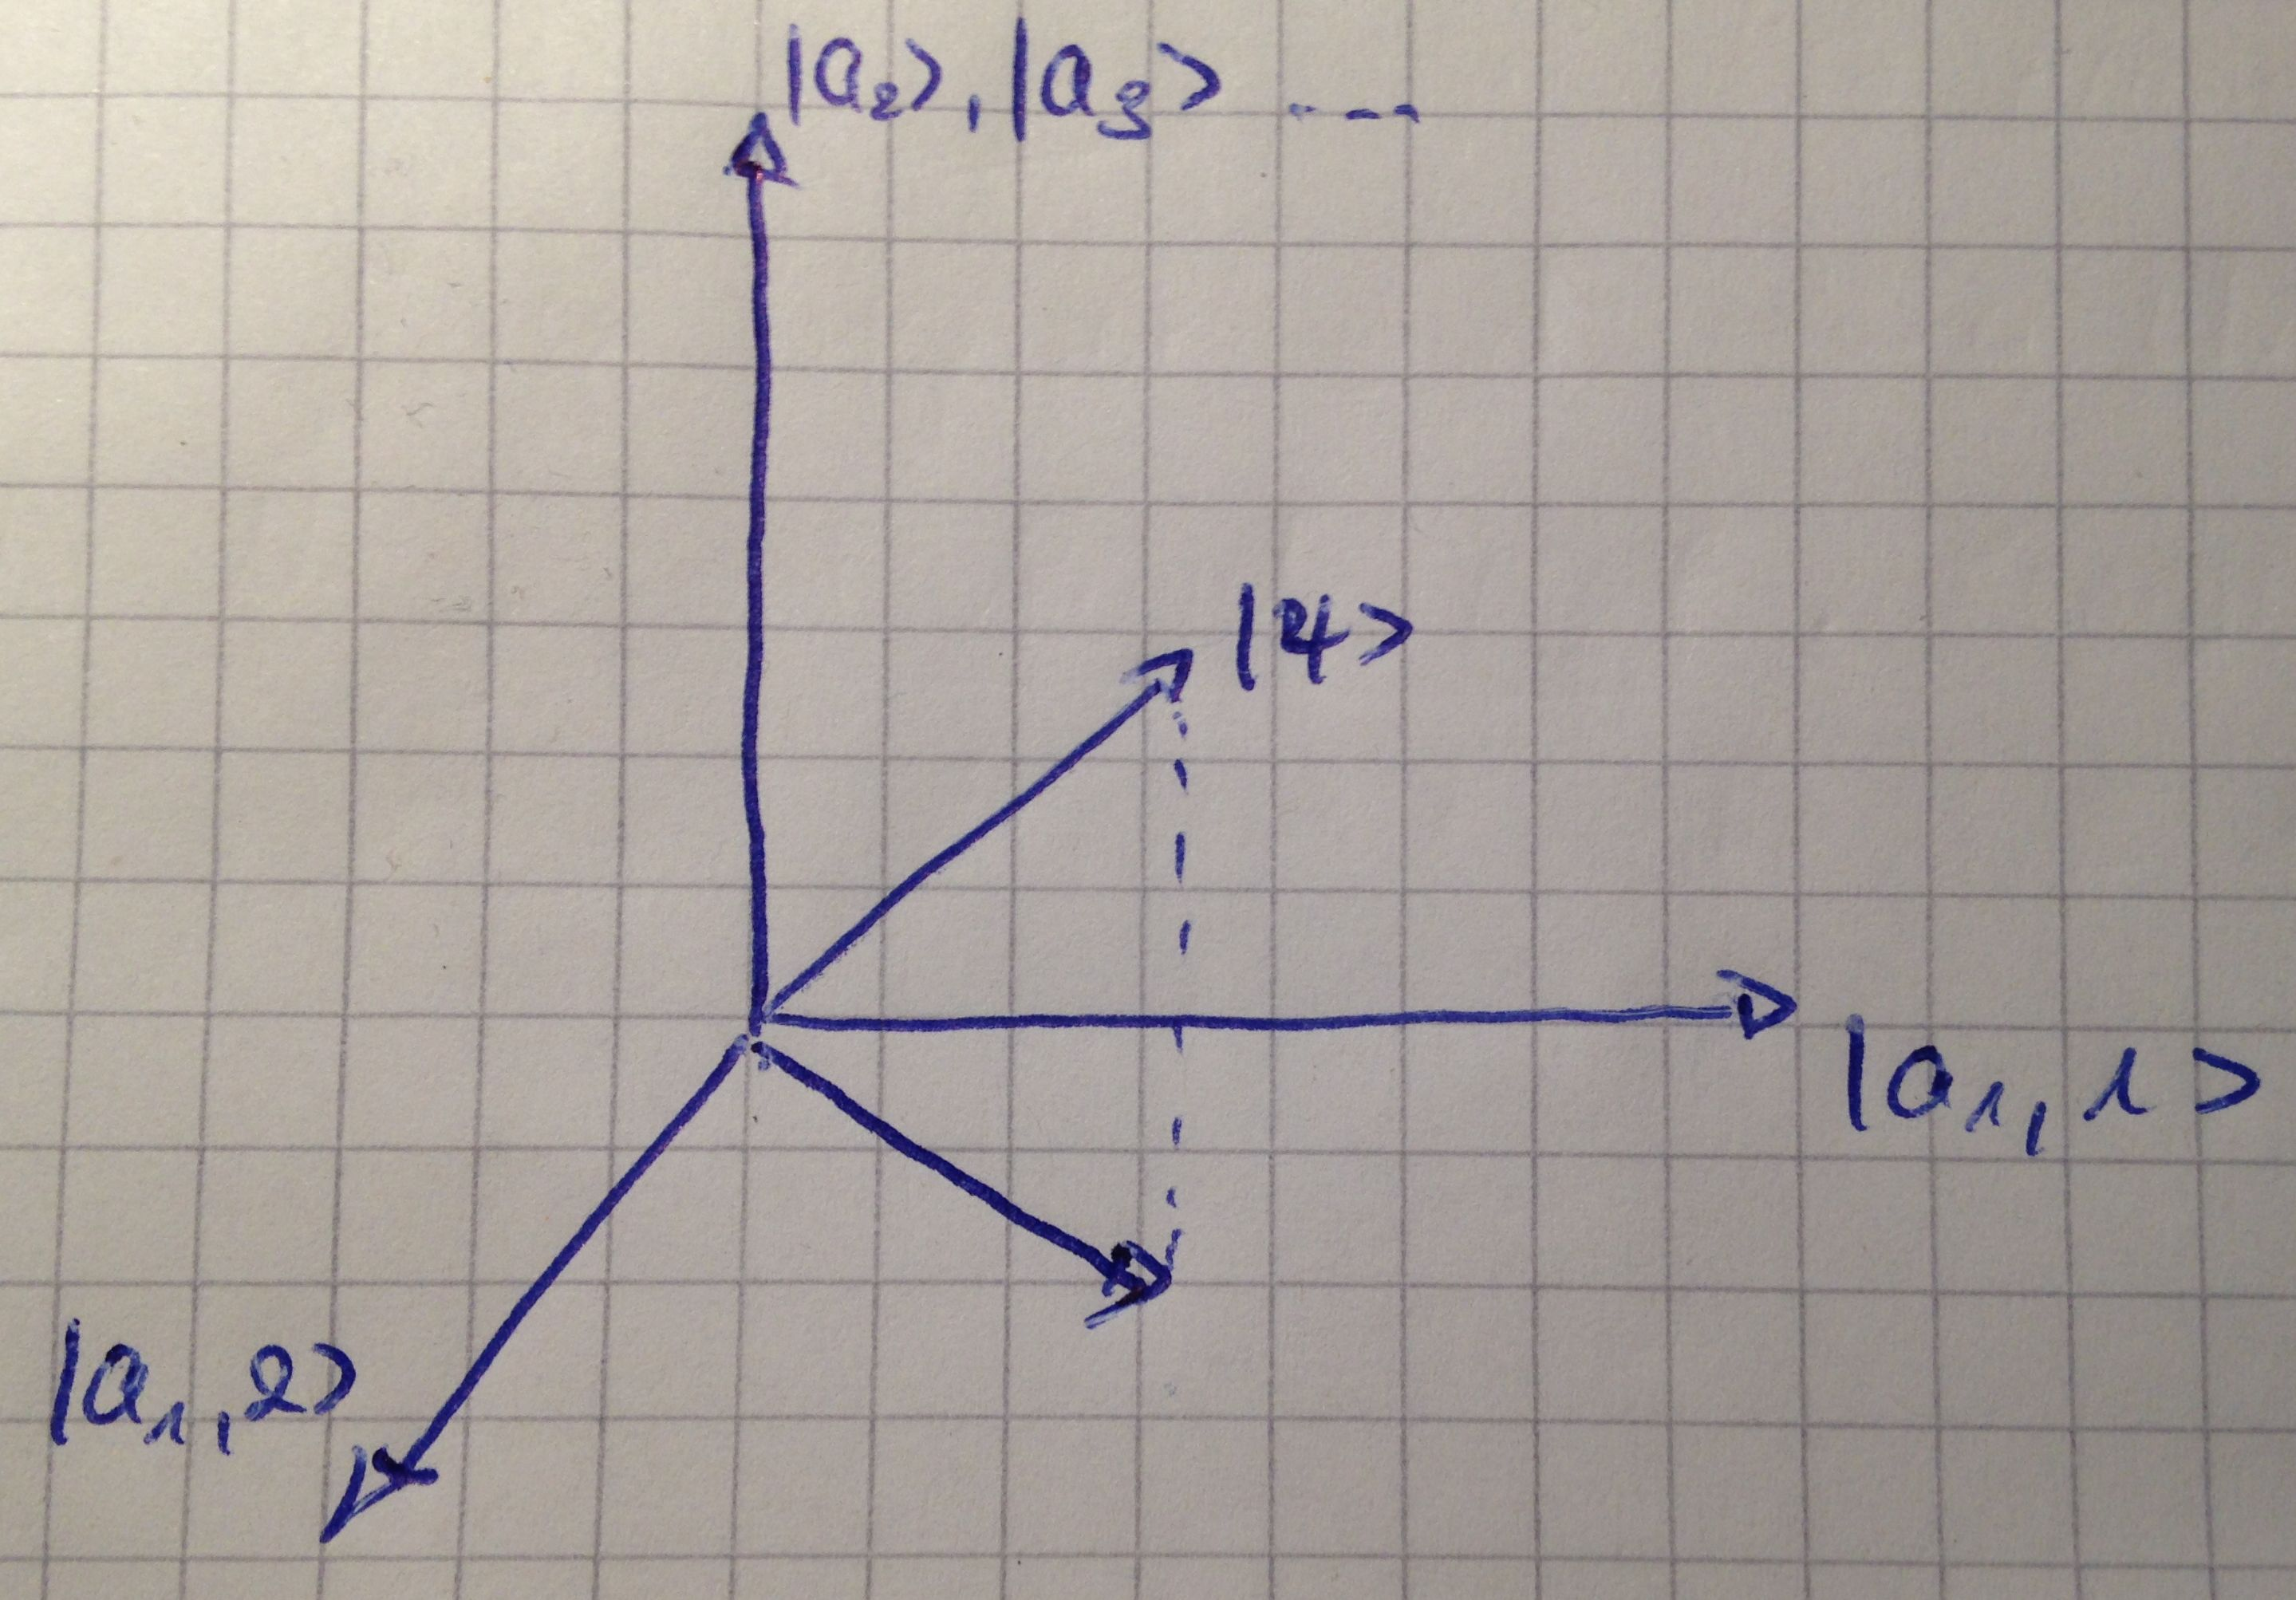
\includegraphics[width=0.7\textwidth]{Messung2}
		\end{center}
	\end{figure}
	
	Eventuelles Problem: Messung von $B$, mit $[\hat{A}, \hat{B}] = 0$
	
	Unabhängig von diesem eventuellen Problem ist
		\begin{align*}
			\hat{\rho}_{\text{red}} &= 
			\sum_m \mathrm{Sp}\, (\hat{P}_{\ket{\psi}} \hat{P}_m) \hat{P}_m =
			\sum_m \hat{P}_m \ket{\psi} \bra{\psi} \hat{P}_m 
		\end{align*}
	Nebenbemerkung 2: Was passiert, wenn man mit einem Gemisch anfängt
		\begin{align*}
			\hat{\rho}_{\text{red}} = \sum_m \hat{P}_m \hat{\rho}_0 \hat{P}_m.
		\end{align*}
	\begin{tabular}{l | l | l}
			Vor der Messung & Nach Messung & Nach Beobachtung des Messergebnisses \\
			\hline  
			$\ket{\psi} = \sum_n c_n \ket{\psi}$
			& -- & 
			$\ket{a_m}$ (rein) (oder Liddersprojektion)
			\\
			$\hat{\rho}_0 = \hat{P}_{\ket{\psi}} (\text{rein})$
			&
			$\hat{\rho}_{\text{red}} = \sum_m \hat{P}_m \hat{P}_{\ket{\psi}} \hat{P}_m$
			& 
			$\hat{\rho}_B = \hat{P}_m$ oder $ \ket{a_m }\bra{a_m}$
			\\
			 & 
			$= \sum_m \mathrm{Sp}\,  (\hat{P}_{\ket{\psi}} \hat{P}_m) \hat{P}_m =
			\sum_m |c_m|^2 \hat{P}_m$  
			& 
			\\
			&
			Gemisch
			&
	\end{tabular} \\
	
	Behauptung: Unitäre Zeitentwicklung lässt reine Zustände rein und verwandelt Gemische in Gemische.
	
	Beweis: 
		\begin{enumerate}[(a)]
			\item \begin{align*}
				\ket{\psi (t)} &= \U (t) \ket{\psi(t)} \\
				\hat{\rho}(t) &= \ket{\psi(t)} \bra{\psi (t)} = 
				\U (t) \hat{\rho}(0) \U^\dagger (t) \\
				\mathrm{Sp}\, ((\hat{\rho}(t))^2) &= 
				\mathrm{Sp}\, ((\U (t) \hat{\rho} (0) \U^\dagger(t))^2) = 1 
			\end{align*}
			\item \begin{align*}
				\hat{\rho}(0) &= \sum_j W_j \ket{\psi_d (0)} \bra{\psi_d (0)} \\
				\hat{\rho}(t) &= \sum_d W_d \U (t) \ket{\psi_d (0)} \bra{\psi_d (0)}
				\U^\dagger(t) =
				\U(t) \left(
					\sum_d W_d \ket{\psi_d (0)} \bra{\psi_d (0)}
				\right) \U^\dagger(t) \\
				\mathrm{Sp}\, ((\hat{\rho}(t))^2) &= 
				\mathrm{Sp}\, ((\hat{\rho}(0))^2) < 1
 			\end{align*}
		\end{enumerate}
	John von Neumann:
		\begin{enumerate}[1.]
			\item Unitäre Zeitentwicklung durch die Schrödinger Gleichung
			\item Zustandsreduktion bei Messungen, nicht - unitär
		\end{enumerate}
	Wir haben $S$ als isoliertes System betrachtet, bei einer Messung gibt es aber Wechselwirkungen mit dem Messgerät.
	
	Zustand des Messapparates vor der Messung $\ket{M_0}$ 
	(Dies ist stark vereinfacht, da Messapparat im Allgemeinen ein statistisches Gemisch ist)
	
	Produktraum der Zustände von $S + M$:
		\begin{align*}
			\ket{\psi} \otimes \ket{M} &= \ket{\psi, M_0}
		\end{align*}
	Erster Zustand von $S$, zweiter Messgerät vor der Messung
	
	Falls $\ket{\psi}$ im Zustand $\ket{a_k}$ gemessen wird, ist $M$ im Zustand $\ket{M_k}$ ( nach der Messung) 
		\begin{align*}
			\ket{a_k, M_0} \underset{Messung}{\longmapsto} \ket{a_k, M_k}
			= \ket{a_k} \otimes \ket{M_k}
		\end{align*}
	Annahme $\braket{M_k | M_\ell} = \delta_{k\ell}$
		\begin{align*}
			\ket{\psi, M_0} = \sum_m c_m \ket{a_m, M_0} \overset{Messung}{\longmapsto}
			\sum_m c_m \ket{a_m, M_m}
		\end{align*}
	$c_m = \braket{a_m | \psi}$
	
	$\ket{a_m, M_0} = (\sum_m c_m \ket{a_m}) \otimes \ket{M_0}$ faktorisiert
	
	$\sum_m c_m \ket{a_m, M_m} = \sum_m c_m (\ket{a_m} \otimes \ket{M_0})$ faktorisiert nicht
	\begin{align*}
		\hat{\rho}_0 \mapsto \hat{\rho}_k &=
		\sum_{m,n} c_m c^*_n \ket{a_m, M_m} \bra{a_n, M_n} =
		\sum_m |c_m|^2 \ket{a_m| M_m }\bra{a_n, M_n} + \text{Interferenzterm}
	\end{align*}
	Wie kommen wir zum Gemisch
		\begin{align*}
			\sum_m |c_m|^2 \ket{a_m, M_m} \bra{a_m, M_m} ?
		\end{align*}
%	Was passiert mit der Interferenztermen?
	
%	Ist Messapparat QM Natur?
%	
%	Ist Messapparat makroskopisch, sollte er den Gesetzen der klassischen Physik folgen.
%	
	Ist Messapparat ``quantenmechanisch''? \marginpar{18.01.2016}Ist dann eine Superposition von Zeigerstellungen denkbar?
	
	Ist Messapparat ``makroskopisch'', dann sollte er den Gesetzen der klassischen Physik folgen. Interferenzterme??
	
	\begin{enumerate}[1)]
		\item Interferenzterme sind sehr klein :
			\begin{align*}
				\braket{M_n | \hat{B} | M_m} &\approx 0 &\text{ für eine Messgröße }B \text{ und } m\neq n
			\end{align*}
			Das hat was mit der ``Irreversibilität'' der Aufzeichnung zu tun. Interferenz ist auch im Prinzip ``da'', wenn kombiniertes System $S + M$ abgeschlossen ist.
		\item Realität: $S + M$ sind nie ganz abgeschlossen. Messgerät $M$ wechselwirkt mit der Umgebung (z.B. Strahlungsfelder) $\Rightarrow$ Vernichtung von Interferenztermen. (``Dekohärenz'')
	\end{enumerate}
Unterschiedliche Vorstellungen davon, was ein ``Zustand'' ist:
	\begin{enumerate}[1)]
		\item Unser Wissen über ein System $\Rightarrow$ ``Sprünge'' nach Messungen sind natürlich, gehorchen aber Gesetzen der klassischen Physik.
		\item $\ket{\psi}$ repräsentiert System selbst.
		
		Was ist dann eine ``ideale'' Messung?
		
		Messprozess ist prinzipiell unsymmetrisch.
		
		Das Messinstrument ist immer ``klassischer'' als das gemessene System, d.h. Interferenzen von $S + M$ sind unterdrückt, relativ zu $S$. 
	\end{enumerate}	 
Egal, ob wir betrachten 
	\begin{align*}
		S &| M, M', B ,& S , M&| M', B ,& S, M, M'&| B
	\end{align*}
``Schnitt'' mit ``Reduktion'' ist immer vorhanden.

$\overset{?}{\Rightarrow}$ Wellenfunktion es Universums inklusive $B$. Wer ist dann Beobachter? Was ist Realität?
	\begin{itemize}
		\item Viel-Welten Interpretation (Everett und Anderen)
			\begin{align*}
				\ket{\psi} = \sum_{i,j} \psi_{ij} \ket{\chi_i} \ket{\phi_j}
			\end{align*}
		$\psi_{ij}$ soll ein relativer Zustand sein
			\begin{align*}
				\sum_j \psi_{ij} \ket{\phi_j} \text{ bzgl. } \ket{\chi_i}
			\end{align*}
		Problem: Zerlegung von $\ket{\psi}$ ist nicht eindeutig. Beispiel
			\begin{align*}
				\ket{\downarrow}, \ket{\uparrow} \text{ oder } \ket{\rightarrow}, \ket{leftarrow} 
			\end{align*}
		$\Rightarrow$ Consistent Histories Approach
		\item Verborgene Parameter: $\ket{\psi}$ enthält nicht die gesamte Information über das System (De Broglie, Bohm) Könnte Determinismus wiederherstellen?
		
		Lässt sich experimentell testen (Bell-Ungleichungen)
	\end{itemize}